\documentclass[10pt]{beamer}

\mode<presentation> {

\usetheme{Madrid}  % Circles & dense

\setbeamertemplate{headline}{%
\leavevmode%
  \hbox{%
    \begin{beamercolorbox}[wd=\paperwidth,ht=2.5ex,dp=1.125ex]{palette quaternary}%
    \insertsectionnavigationhorizontal{\paperwidth}{}{\hskip0pt plus1filll}
    \end{beamercolorbox}%
  }
}

\setbeamertemplate{navigation symbols}{}

}

\setbeamertemplate{caption}[numbered]

\usepackage{graphicx}
\usepackage{booktabs}
\usepackage{fontspec}
\usepackage{amsmath}
\mathchardef\mhyphen="2D % Define a "math hyphen"
\usepackage{caption}
\usepackage{xunicode}
\usepackage{xltxtra}
\usepackage{lipsum}
\usepackage{xecyr}
\usepackage{hyperref}
\usepackage{amsthm}
\usepackage{blindtext}
\usepackage{makecell}
\usepackage{multirow}
\usepackage{array}
\usepackage{siunitx}
\usepackage{booktabs}
\usepackage{bigdelim}
\usepackage{multicol}

\usepackage{polyglossia}
\setdefaultlanguage{english}
\setotherlanguages{russian}
\setmainfont[Mapping=tex-text]{CMU Serif}
\setsansfont[Mapping=tex-text]{CMU Sans Serif}
\setmonofont[Mapping=tex-text]{CMU Serif}

\newread\tmp
\openin\tmp=main.bib%
\read\tmp to \bib%
\closein\tmp%
\begin{filecontents}[overwrite]{\jobname.bib}
\bib
\end{filecontents}
\usepackage[style=verbose,backend=biber]{biblatex}
\addbibresource{main.bib}

\definecolor{green}{RGB}{0, 200, 0}

\addto\captionsenglish{%
  \renewcommand{\figurename}{Фигура}%
  \renewcommand{\tablename}{Таблица}%
}

\title[Генерация речи]{TalkNet: Конволюционная неавторегрессионая модель для задачи генерации речи}
\author[Беляев Станислав]{Беляев Станислав Валерьевич\\\footnotesize\textcolor{gray}{Научный руководитель: Гинзбург Б.Е.}{}}
\institute[НИУ ВШЭ]{Санкт-Петербургская школа физико-математических и компьютерных наук\\~\\НИУ ВШЭ -- Санкт-Петербург}
\date{16 июня 2020}

\begin{document}

\begin{frame}
\titlepage
\end{frame}

\section{Введение}

\begin{frame}{Постановка задачи}
\begin{block}{Задача генерации речи (Text-To-Speech, TTS)}
    По входному тексту сгенерировать аудиодорожку с человеческой речью.
\end{block}
Обычно разделяют на две части: генерация мэл-спектрограммы (компактное, вычислимое и детерменированное представление аудио) и вокодинг:
\begin{figure}[H]
\centering
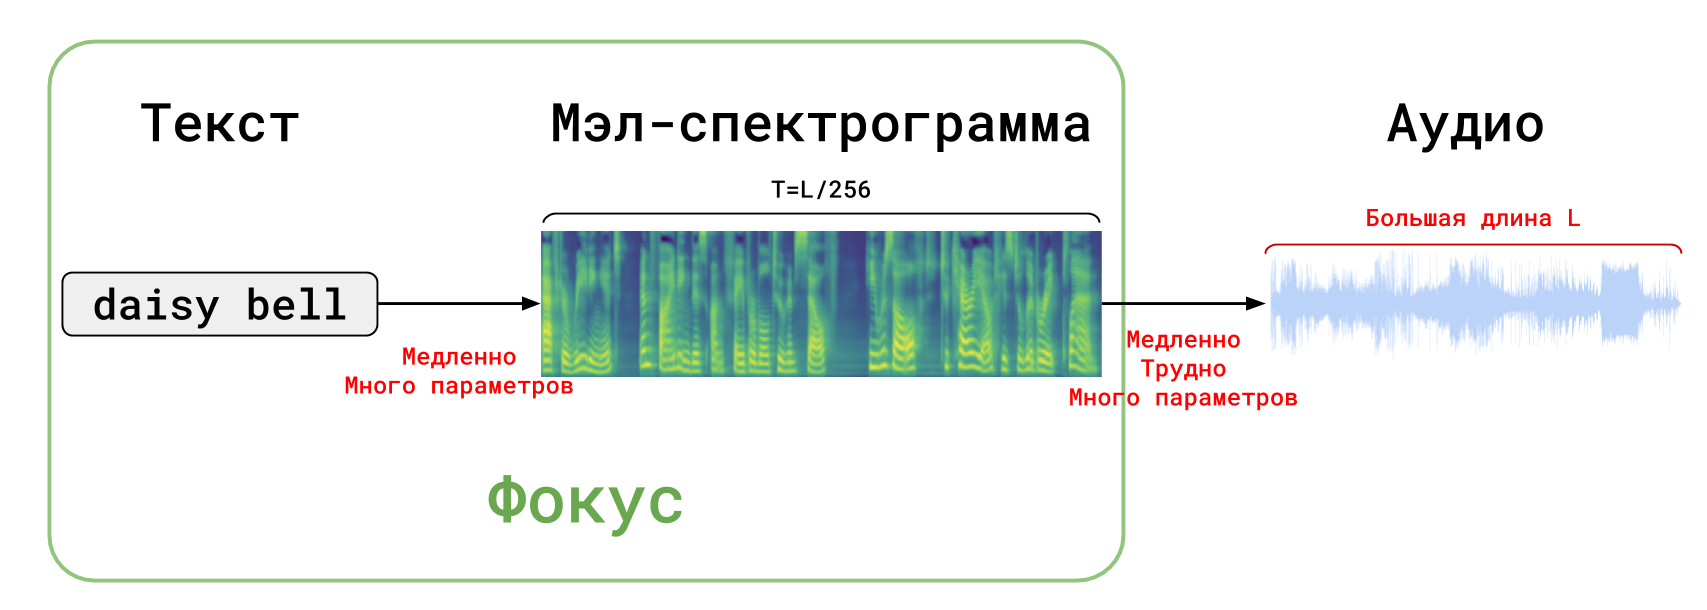
\includegraphics[width=1.0\textwidth]{images/tts-pipeline-rus.png}
\caption{Современный двухшаговый пайплайн генерации речи из текста}
\end{figure}
\end{frame}

\begin{frame}{Обзор существующих решений}
\begin{block}{Устойчивость (robustness)}
    Способность процесса генерации избегать запинаний и пропуска букв/слов.
\end{block}
\vspace{-0.5cm}
\begin{columns}[T]
\begin{column}{0.5\textwidth}
\begin{center}
\renewcommand{\thefootnote}{1,2}
\textbf{Авторегрессионные методы}\footnotemark\\
Cлева направо, шаг за шагом
\end{center}
\begin{figure}[H]
\centering
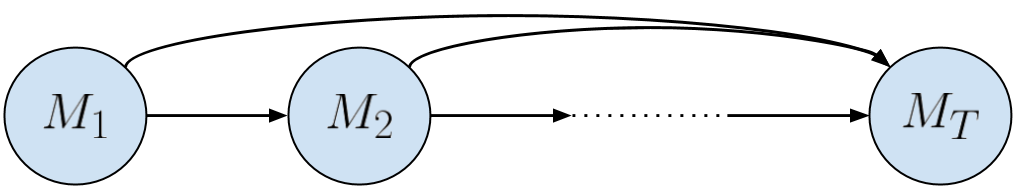
\includegraphics[width=0.8\textwidth]{images/methods/areg.png}
\end{figure}
\begin{itemize}
    \item[] \textcolor{red}{- Медленное обучение и генерация}
    \item[] \textcolor{red}{- Отсутствие устойчивости}
    \item[] \textcolor{red}{- Много обучаемых параметров}
    \item[] \textcolor{green}{+ Хорошее качество}
\end{itemize}
\end{column}
\begin{column}{0.5\textwidth}
\begin{center}
\renewcommand{\thefootnote}{3}
\textbf{Неавторегрессионные методы}\footnotemark\\
Параллельно
\end{center}
\begin{figure}[H]
\centering
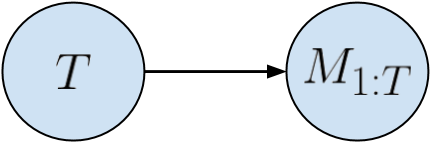
\includegraphics[width=0.47\textwidth]{images/methods/nareg.png}
\end{figure}
\begin{itemize}
    \item[] \textcolor{green}{+ Быстрое обучение и генерация}
    \item[] \textcolor{green}{+ Устойчивость}
    \item[] \textcolor{red}{- Много обучаемых параметров}
    \item[] \textcolor{red}{- Чуть хуже качество}
\end{itemize}
\end{column}
\end{columns}
\renewcommand{\thefootnote}{1}
\footcitetext{tacotron2}
\renewcommand{\thefootnote}{2}
\footcitetext{transformer-tts}
\renewcommand{\thefootnote}{3}
\footcitetext{fastspeech}
\end{frame}

% \begin{frame}{Обзор существующих решений}
% Подходы разделяют на два класса - авторегрессионный (слева направо по времени) и неавторегрессионные (параллельная генерация).
% \begin{itemize}
%     \item Tacotron2~\footcite{tacotron2}: 30M весов, медленный авторегрессионный вывод (RNN), проблема с устойчивостью (пропуск слов и запинания), хорошее качество.
%     \item Transformer-TTS~\footcite{transformer-tts}: 60M весов, медленный авторегрессионный вывод, проблема с устойчивостью, хорошее качество.
%     \item FastSpeech~\footcite{fastspeech}: 30M весов, параллельная генерация, проблемы с обобщением на другие языки, использует Tacotron2 для извлечения данных для обучения (teacher model).
% \end{itemize}
% Все существующие подходы используют механизм внимания (attention), время работы которого зависит квадратично от длины мэл-спектрограммы и имеют 30M+ обучаемых параметров.
% \end{frame}

% \begin{frame}{Неавторегрессионность}
% \begin{figure}[H]
% \centering
% 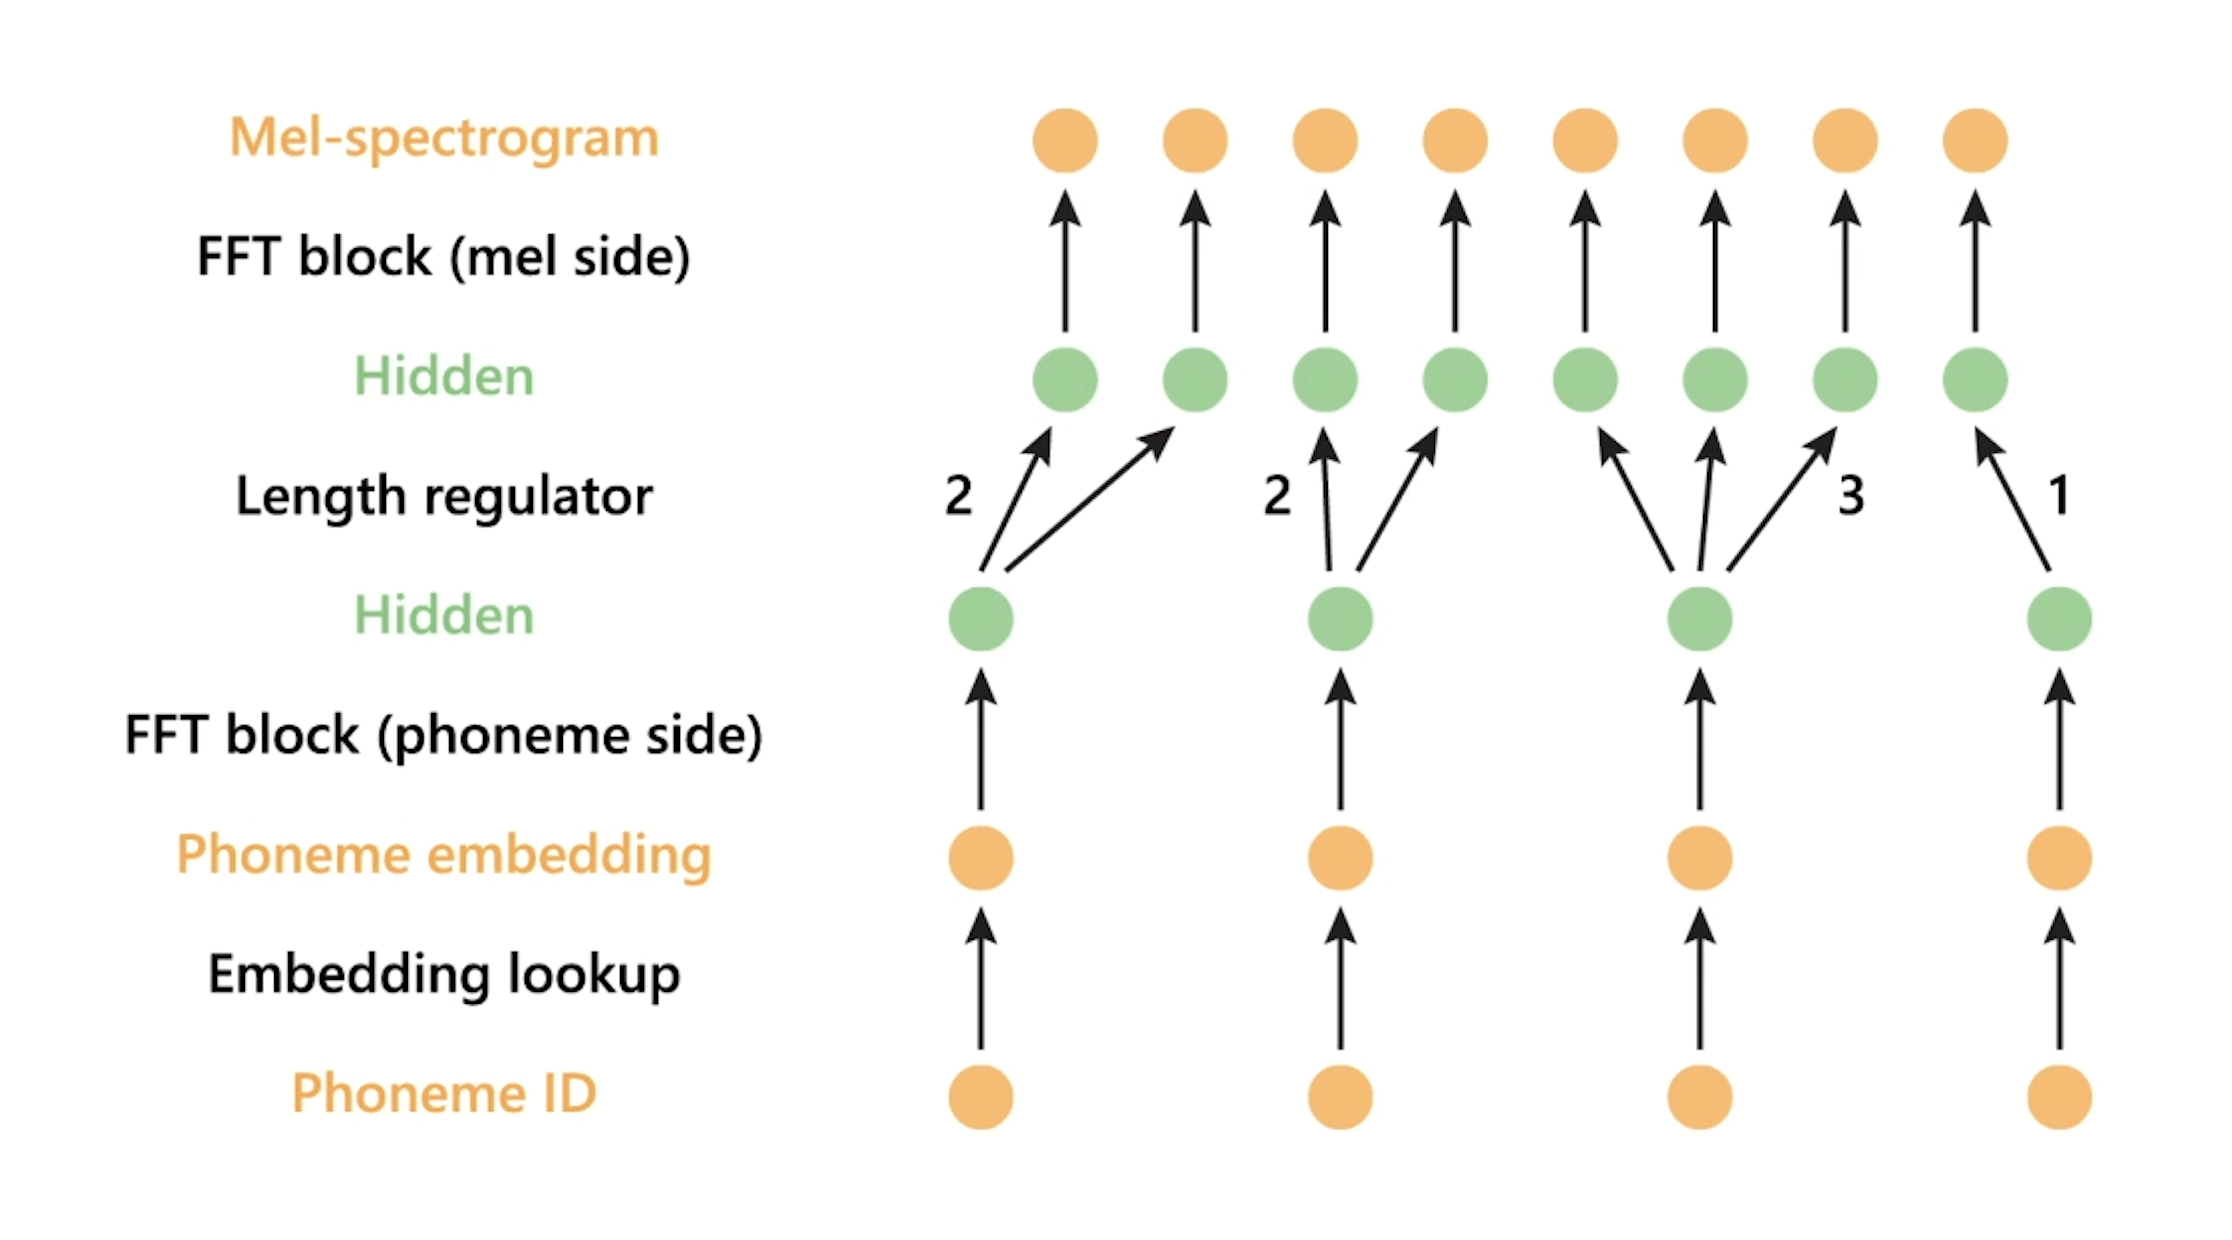
\includegraphics[width=1.0\textwidth]{images/fastspeech/alignment.png}
% \end{figure}
% \end{frame}

\section{Цели и задачи}

\begin{frame}{Цели и задачи}
\begin{block}{Цель}
    Целью данной работы является разработка нового подхода для задачи синтеза речи, позволяющего производить \textbf{быструю, качественную и устойчивую} генерацию с \textbf{малым} количеством обучаемых параметров.
\end{block}
\vspace{0.4cm}
Задачи:
\begin{itemize}
    \item Разработать и описать эффективную нейронную архитектуру, основанную на идеи неавторегрессионности.
    \item Выбрать данные для обучения, провести эксперименты и замерить результаты.
    \item Произвести сравнение качества и устойчивости генерации с существующими решениями.
    \item Проанализировать скорость генерации и сравнить с другими подходами.
\end{itemize}
\end{frame}

\section{Решение}

\begin{frame}{Идея}
\begin{block}{Длительность символа}
    Количество шагов в спектрограмме, соответствующих выводу символа.
\end{block}
\vspace{-0.1cm}
\begin{figure}[H]
\centering
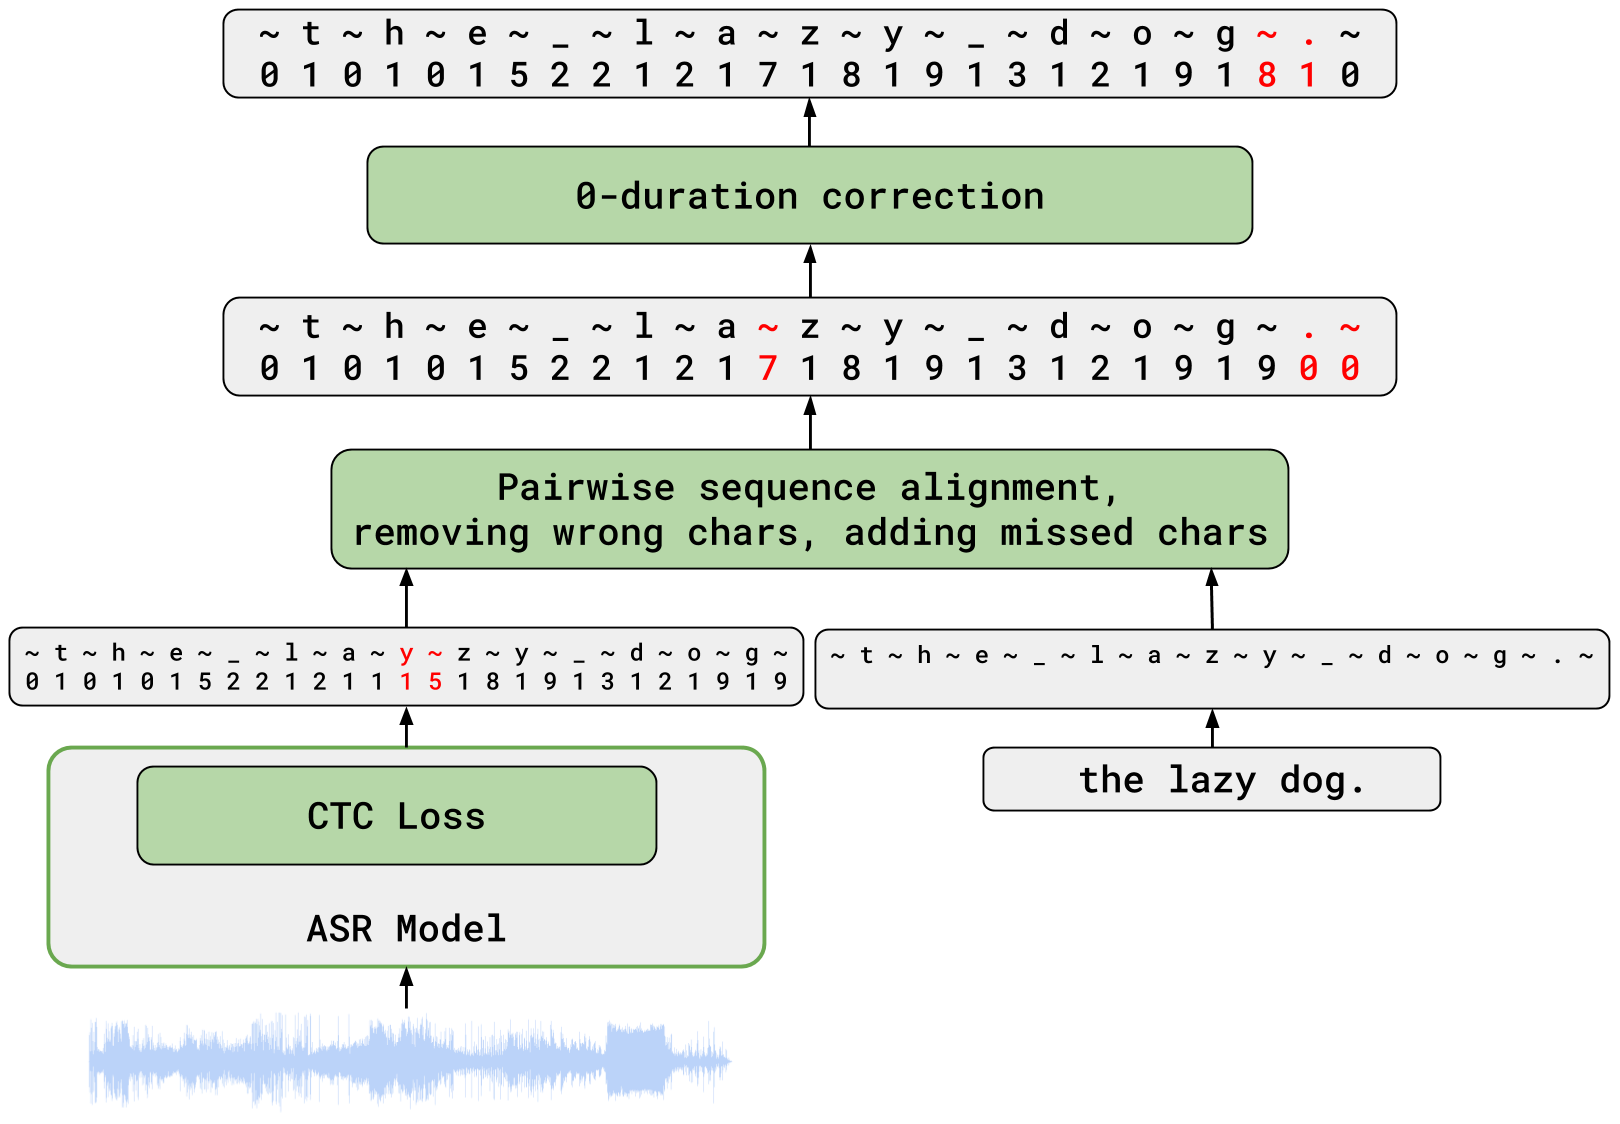
\includegraphics[width=0.47\textwidth]{images/alignment.png}
\caption{Временное выравнивание текста и аудио}
\end{figure}
\vspace{-0.4cm}
\begin{itemize}
    \item Зная истинные длительности всех символов, можно построить \textbf{неавторегрессионный} генератор мэл-спектрограммы. Хорошее выравнивание позволяет получить свойство \textbf{устойчивости}.
    \item Длительности датасета можно извлечь из модели, решающей обратную задачу -- разпознования речи (Automatic Speech Recognition, ASR).
    \item Этап предсказания длительностей для символов входного текста требует отдельной \textbf{неавторегрессионной} нейронной модели.
\end{itemize}
\end{frame}

% \begin{frame}{Идея}
% \begin{itemize}
%     \item Разделить генерацию на два парралельных этапа: предсказывание длительностей графем и генерацию мэл-спектрограммы.
%     \item Истинные длительности для обучения предсказателя достать из обратной задачи -- разпознавания речи (ASR). Модель QuartzNet~\footcite{quartznet}, основанная на применении функции ошибки СТС, явным образом учит выравнивание мэла на текст.
%     \item Введение дополнительного символа ($\sim$), обозначающего промежуточное состояние между соседними символами.
%     \item Конволюционная архитектура позволяет добиться малого количества параметров.
% \end{itemize}
% \end{frame}

\begin{frame}{Архитектура}
\begin{figure}[H]
\centering
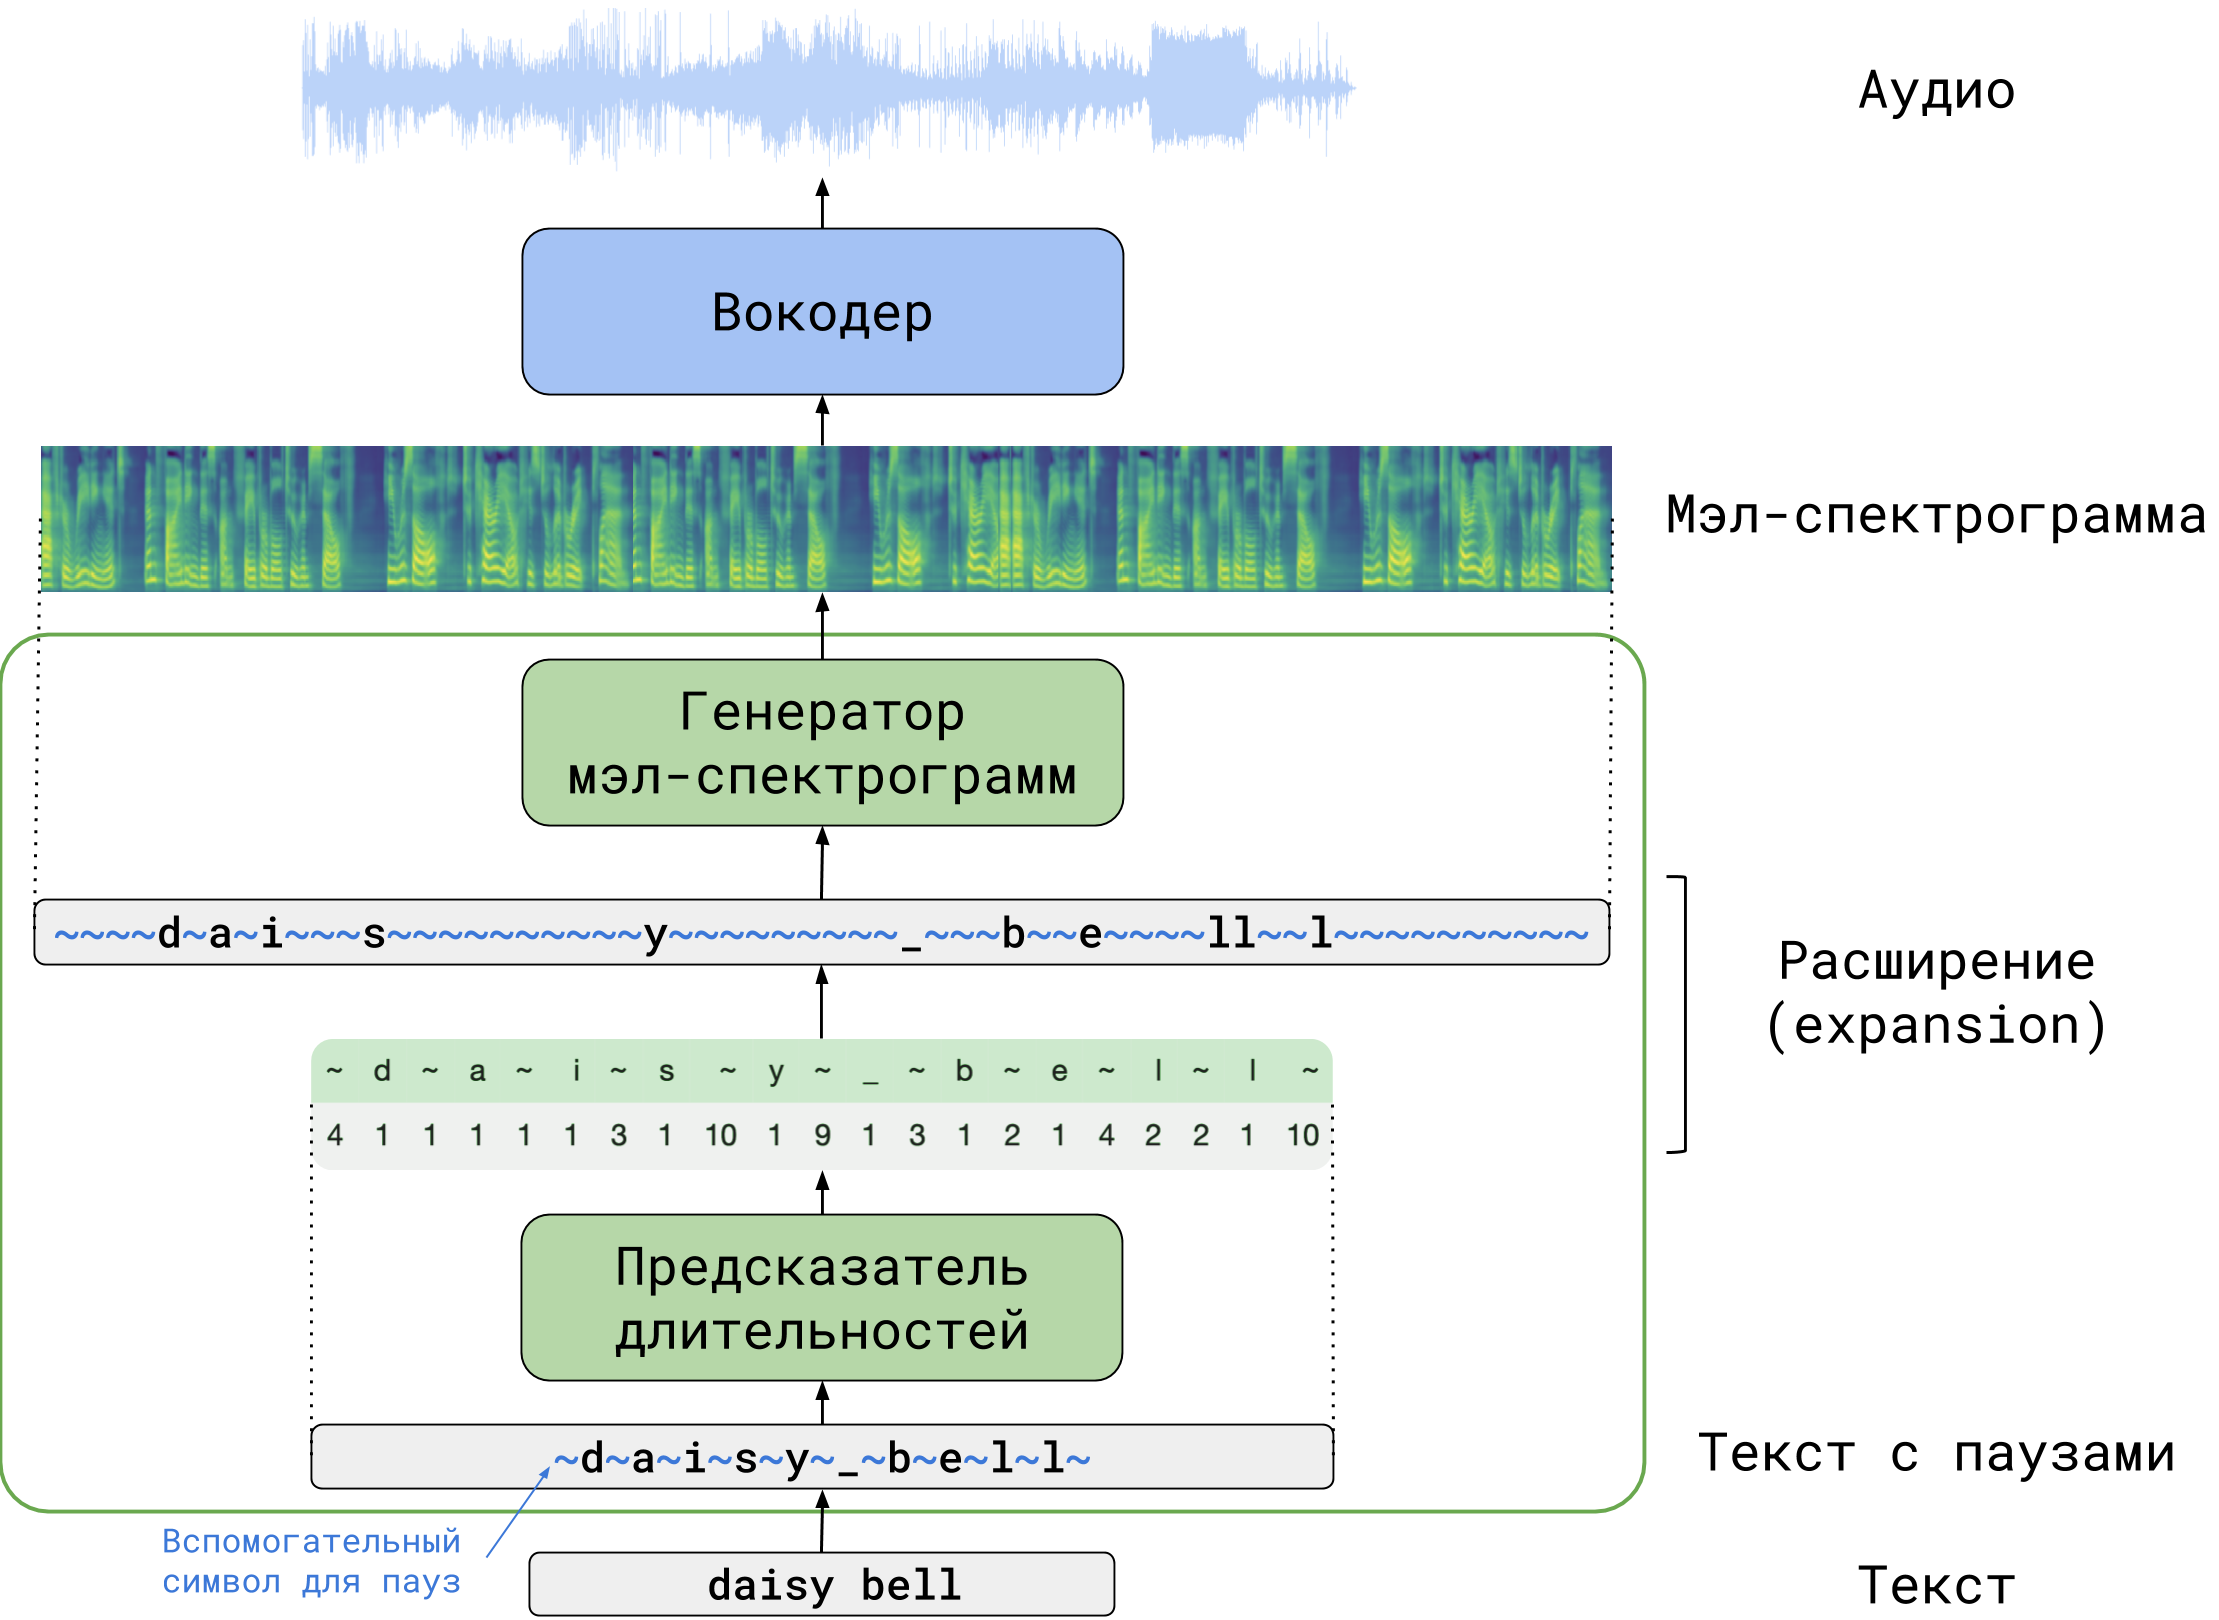
\includegraphics[width=0.8\textwidth]{images/arch-rus.png}
\caption{Архитектура генерации аудио TalkNet}
\end{figure}
\end{frame}

\begin{frame}{Извлечение истинных длительностей}
\renewcommand{\thefootnote}{4}
\begin{figure}[H]
\centering
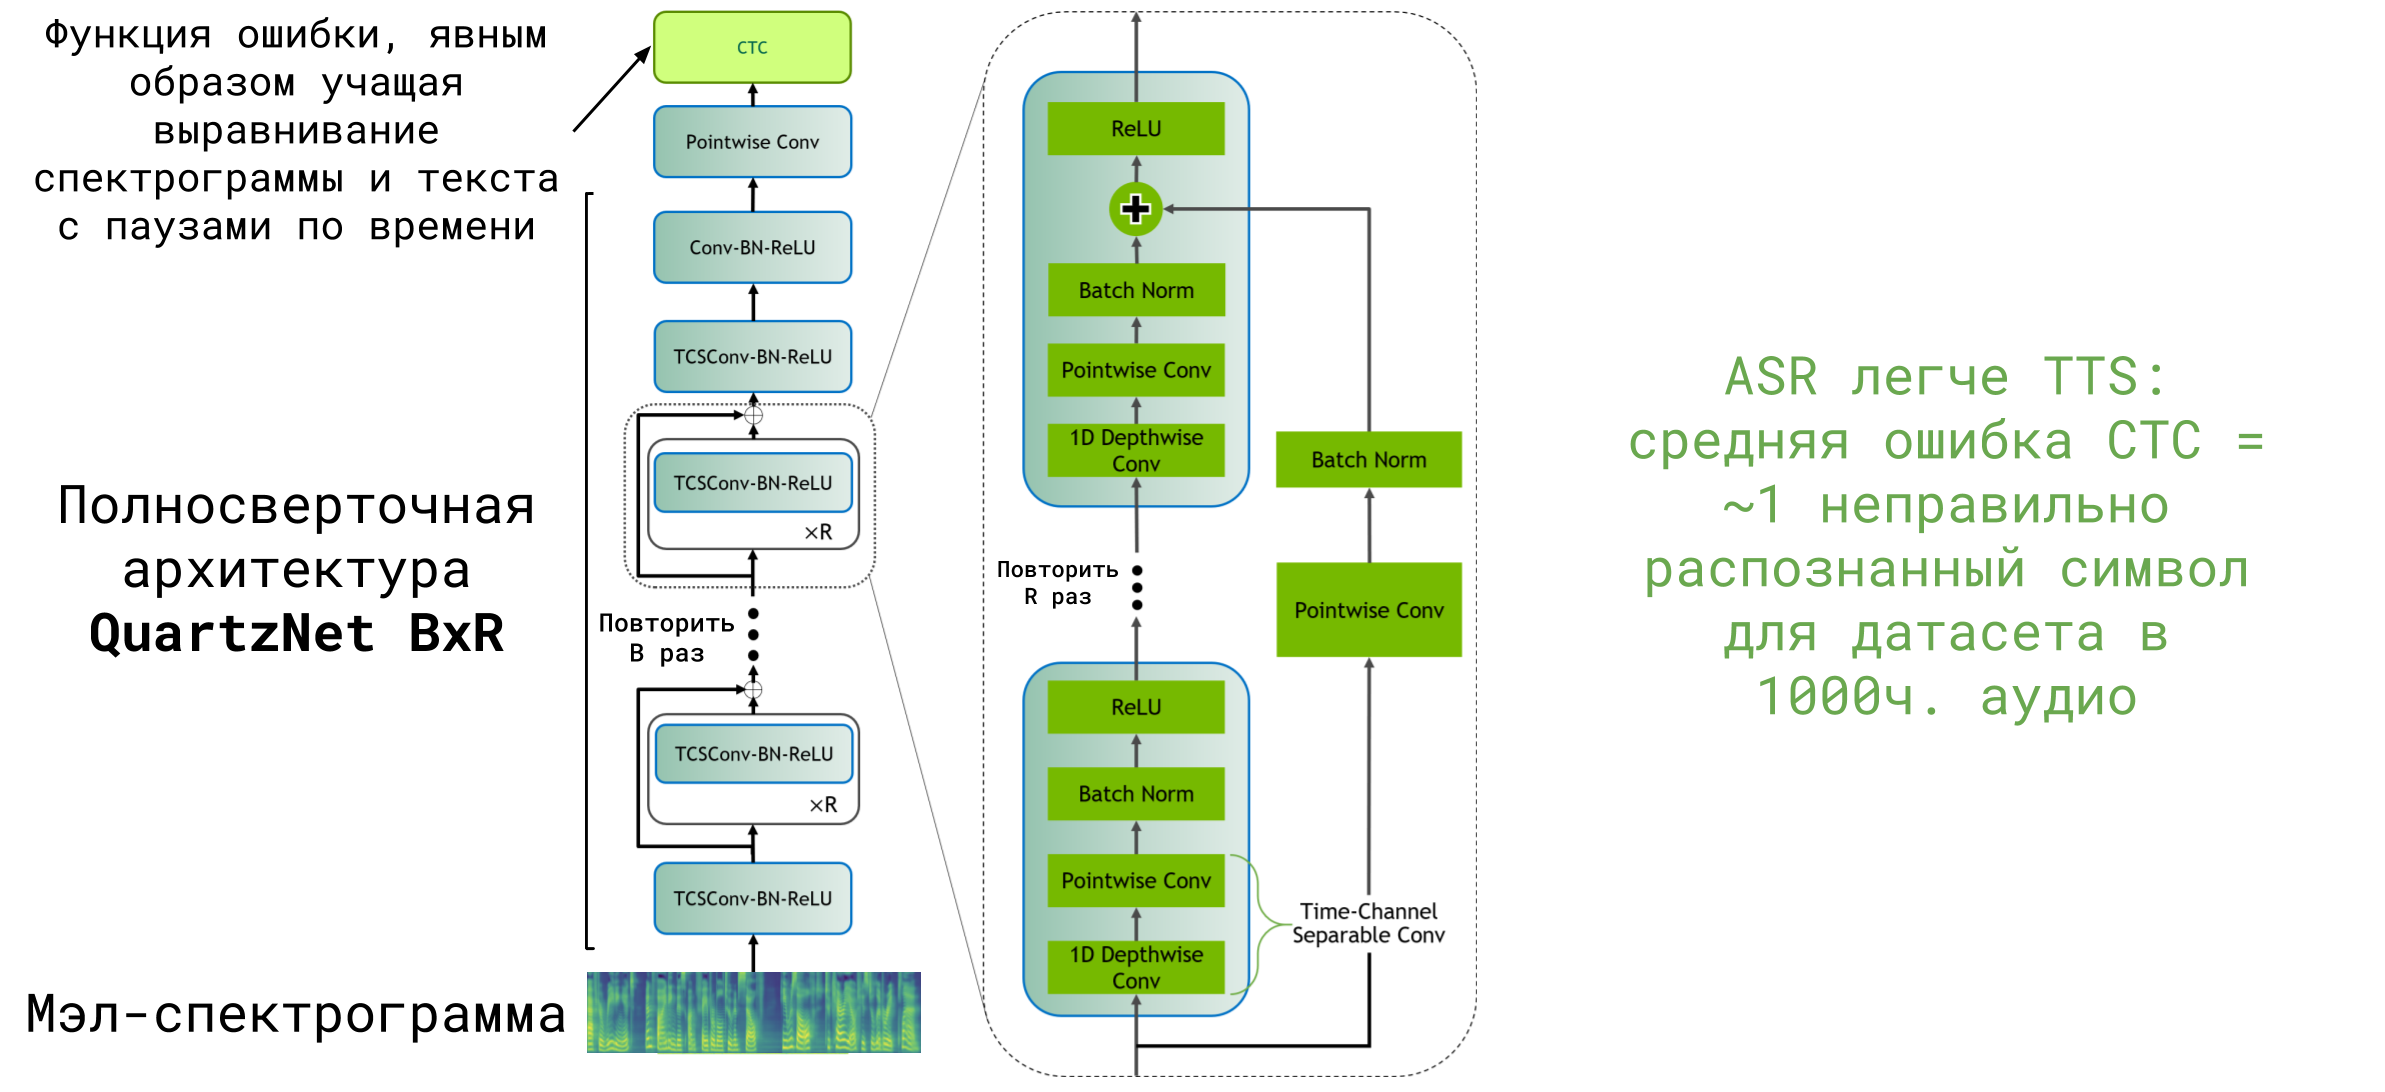
\includegraphics[width=1.0\textwidth]{images/qn-rus.png}
\caption{QuartzNet~\footcite{quartznet} решает обратную задачу: разпознавания текста по аудио. Функция ошибки учит выравнивание, из которого извлекаются длительности букв.}
\end{figure}
\end{frame}

% \begin{frame}{Извлечение истинных длительностей}
% \begin{figure}[H]
% \centering
% 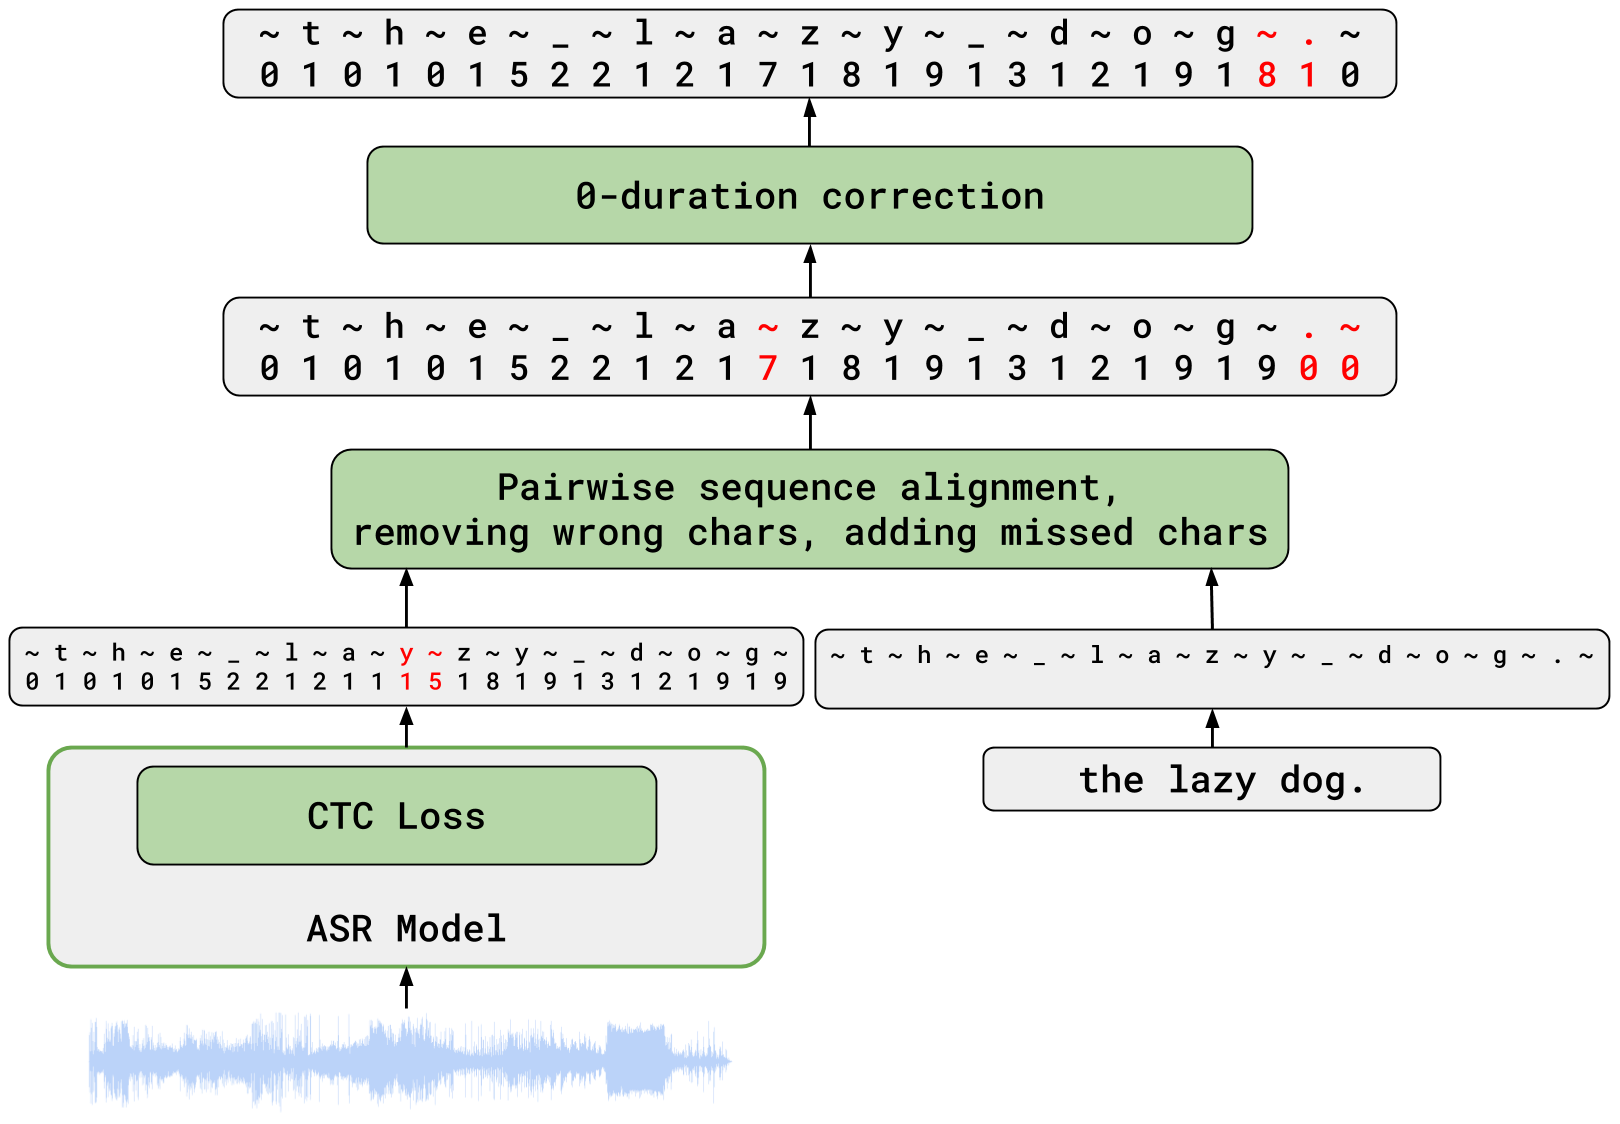
\includegraphics[width=0.9\textwidth]{images/extraction.png}
% \end{figure}
% \end{frame}

\begin{frame}{Процесс обучения}
\renewcommand{\thefootnote}{5}
\begin{table}[!ht]
\centering
\scalebox{1.0}{
\begin{tabular}{l c c c}
\toprule
\textbf{Этап} &
\textbf{Архитектура} &
\textbf{\thead{Количество\\параметров}} &
\textbf{\thead{Время\\обучения}} \\
\midrule
Предсказатель длительностей & QuartzNet 5x5 & 2M & 15м. \\
Генератор спектрограммы & QuartzNet 9x5 & 8M & 2ч. \\
\bottomrule
\end{tabular}
}
\caption{Параметры обучения для двух независимых этапов TalkNet}
\end{table}
\vspace{-0.3cm}
\begin{itemize}
    \item Для обучения использовался набор данных LJSpeech~\footcite{ljspeech} -- 24 часа одноголосой речи из аудиокниг с художественной литературой.
    \item Общее количество обучаемых параметров модели -- \textbf{10M} -- в \textbf{3} раза меньше чем у любого другого современного подхода.
    \item Общее количество времени на обучение -- \textbf{2 часа} -- в \textbf{20} раз быстрее лучших авторегрессионных методов.
    \item Для обучения применялся случайный несмешенный шум для истинных длительностей, что стабилизировало процесс и повысило качество.
\end{itemize}
\end{frame}

\section{Сравнение}

\begin{frame}{Сравнение качества}
\begin{block}{Mean Opinion Score (MOS)}
    Слепая оценка носителей языка натуральности речи предложенного аудио по дискретной шкале от $1.0$ до $5.0$ с шагом $0.5$. Каждый пример оценивается несколькими разными слушателями для понижения дисперсии.
\end{block}
\begin{table}[!ht]
\centering
\scalebox{1.0}{
\begin{tabular}{l cl} 
\cmidrule[\heavyrulewidth]{1-2}
\textbf{Подход} &
\textbf{MOS} \\
\cmidrule{1-2}
Оригинальное аудио & $4.31 \pm 0.05$ \\
Оригинальный мэл + WaveGlow & $4.04 \pm 0.05$ \\
Tacotron 2 + WaveGlow & $3.85 \pm 0.06$ & \hspace{-0.5em}\rdelim\}{2}{*}[\renewcommand{\theadfont}{\small\bfseries}\thead{Небольшая\\разница}] \\
\cmidrule{1-2}
TalkNet + WaveGlow & $3.74 \pm 0.07$ \\
\cmidrule[\heavyrulewidth]{1-2}
\end{tabular}
}
\caption{Оценки MOS с использованием вокодера WaveGlow и $95\%$ доверительным интервалом. Оценки усреднялись по 100 примерам, каждый из которых был оценен не менее 10 раз. Как можно заметить, \textbf{качество TalkNet сравнимо с Tacotron 2} -- авторегресионным подходом, считающихся одним из лучших на сегодняшний момент.}
\end{table}
\end{frame}

\begin{frame}{Сравнение скорости}
\begin{block}{Latency}
    Количество секунд, требуемых на генерацию одного аудио.
\end{block}
\begin{block}{Real Time Factor (RTF)}
    Количество секунд аудио, генерирующихся за одну секунду вычислений.
\end{block}
\begin{table}[!ht]
\centering
\scalebox{1.0}{
\begin{tabular}{l l l r} 
\toprule
\textbf{Model} & 
% \textbf{Batch} &
\textbf{Latency, с} &
\textbf{RTF} \\
\midrule
Transformer TTS & $6.735 \pm 3.969$ & $1.48 \pm 0.87$ \\
Tacotron 2 & $0.817 \pm 1\cdot 10^{-2} $ & $7.56 \pm 0.01$ \\
FastSpeech & $0.029 \pm 2 \cdot {10}^{-4}$ & $221.01 \pm 1.75$ \\
\midrule
TalkNet & $\mathbf{0.019 \pm 1 \cdot {10}^{-5}}$ & $\mathbf{328.65 \pm 4.76}$ \\
% TalkNet & 4 & $0.023 \pm 5 \cdot {10}^{-5}$ & $1048.80 \pm 21.75$ \\
% TalkNet & 8 & $0.037 \pm 4 \cdot {10}^{-4}$ & $1340.09 \pm 8.90$ \\
\bottomrule
\end{tabular}
}
\caption{Сравнение скорости генерации с $95\%$ доверительным интервалом. Количество примеров для усреднения -- 2048, а средняя длина мэл-спектрограммы -- 540. Как видно, \textbf{TalkNet значительно быстрее} современных методов.}
\end{table}
\end{frame}

\begin{frame}{Генерация за O(1)}
\begin{block}{Механизм внимания (attention)}
    Вычислительная операция для упрощения поиска взаимосвязей в данных, работающая квадратично от времени аудио (длины спектрограммы). Используется \textbf{во всех} современных моделях для генерации речи.
\end{block}
\begin{figure}[H]
\centering
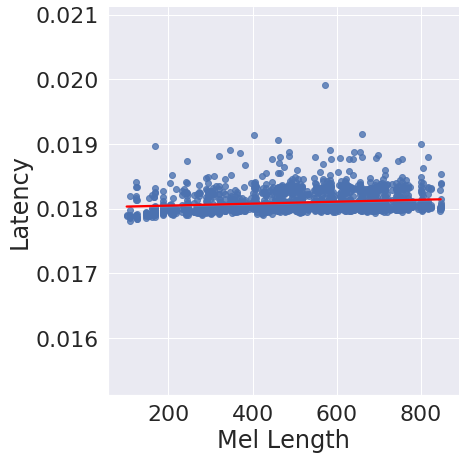
\includegraphics[width=0.35\textwidth]{images/len-lat.png}
\caption{График зависимости длины мэла от latency. Неавторегрессионность и \textbf{отсутствие} механизмов внимания позволяют получить \textbf{константное} время вывода.}
\end{figure}
\end{frame}

\section{Результаты}

\begin{frame}{Результаты}
\begin{itemize}
    \item Разработана \textbf{устойчивая} неавторегрессионная модель для синтеза речи, которая использует предобученную модель задачи разпознавания речи для извлечения истинных длительностей символов.
    \item Подход обладает \textbf{высокой} скоростью обучения (до \textbf{20} раз в сравнении другими моделями) и генерации (в \textbf{320} раз быстрее реального времени). Скорость генерации \textbf{не зависит} от длины входного текста.
    \item Архитектура подхода позволяет \textbf{уменьшить} количество обучаемых параметров до \textbf{10M} -- в \textbf{3} раза меньше по сравнению с конкурентами, показывая при этом \textbf{сравнимое} качество.
    \item \renewcommand{\thefootnote}{6}Статья~\footcite{beliaev2020talknet} (INTERSPEECH 2020)
    \item \renewcommand{\thefootnote}{7}Код~\footnote{\url{https://github.com/NVIDIA/NeMo/tree/master/examples/tts}}
\end{itemize}
\end{frame}

\begin{frame}{Литература}
\begin{columns}
\column{0.8\paperwidth}
\printbibliography[heading=none]
\end{columns}
\end{frame}

\end{document}